\documentclass[aspectratio=169, 11pt, t, usepdftitle=false]{beamer}

% Replication slides: Zhu, Shi & Banerjee (2025), Management Science, Tables 2–4

% ── Template ──────────────────────────────────────────────────
\usepackage{penn-template}

% ── Packages ──────────────────────────────────────────────────
\usepackage{mathtools}
\usepackage{booktabs}
\usepackage{array}
\usetikzlibrary{arrows.meta, positioning, decorations.pathreplacing}

% ── Bibliography ──────────────────────────────────────────────
\usepackage[backend=biber,style=authoryear-comp,natbib=true,maxcitenames=2]{biblatex}
\addbibresource{reference.bib}
\renewcommand*{\bibfont}{\footnotesize}

% ── Appendix frames are not counted ───────────────────────────
\usepackage{appendixnumberbeamer}

% ── Deck helpers ──────────────────────────────────────────────
% Replication columns in UniBlue
\newcolumntype{R}{>{\color{UniBlue}}c}
% Small note under a figure or table
\newcommand{\source}[1]{{\scriptsize\color{TextMid}#1\par}}
% The paper's conclusion for a table: a filled strip in the template's block style
\newmdenv[style=wbBlockBase, linecolor=UniBlue, backgroundcolor=UniBlueLight,
  innertopmargin=0.25em, innerbottommargin=0.3em, innerleftmargin=0.3cm,
  skipabove=0.7em, skipbelow=0.6em]{conclusionbox}
% Column heading on the discussion page: bold blue text over a thin gray rule
\newcommand{\colhead}[1]{%
  {\small\bfseries\color{UniBlue}#1\strut\par}\vspace{0.15em}%
  {\color{DividerGray}\hrule height 0.6pt}\vspace{0.1em}}
\newcommand{\conclusion}[1]{%
  \begin{conclusionbox}\small\textbf{\color{UniBlue}Paper's conclusion:} #1\end{conclusionbox}}
% Equation term with a short label under a brace; the label does not widen the term,
% and the phantom gives every brace the same depth so the labels line up
\newcommand{\explain}[2]{{\underbrace{#1\vphantom{X_{gjp(t)}}}_{\mathclap{\text{\fontsize{6.5}{7.5}\selectfont\color{TextMid}%
  \renewcommand{\arraystretch}{0.85}\begin{tabular}[t]{@{}c@{}}#2\end{tabular}}}}}}
% Tighter space under the frame title and in lists
\addtobeamertemplate{frametitle}{}{\vspace{-0.45cm}}
\makeatletter
\setbeamertemplate{itemize/enumerate body begin}{%
  \def\@listi{\leftmargin\leftmargini \topsep 2\p@ \parsep 0\p@ \itemsep 1.5\p@}}
\makeatother
% TikZ styles: year boxes (Table 2) and chain boxes (discussion)
\tikzset{
  yr/.style={draw=DividerGray, fill=#1, minimum width=2.3cm, minimum height=0.5cm,
             inner sep=0pt, font=\small\bfseries, text=TextDark},
  chain/.style={draw=#1, line width=0.8pt, fill=white, rounded corners=2pt,
                text width=2.25cm, minimum height=0.8cm, align=center,
                font=\scriptsize, text=TextDark},
}

% ── Metadata ──────────────────────────────────────────────────
% The template's title sizes are fixed (24pt / 13.5pt); set smaller ones here,
% and start the title a little higher to leave room for the author block
\title[Replication of Zhu, Shi \& Banerjee (2025)]{%
  \vspace*{-0.4cm}\fontsize{16}{20}\selectfont
  Monetizing Platforms: An Empirical Analysis of\\
  Supply and Demand Responses to Entry Costs\\
  in Two-Sided Markets}
\subtitle{%
  \fontsize{11.5}{15}\selectfont
  {\color{white}Kai Zhu, Qiaoni Shi and Shrabastee Banerjee}\\
  \textit{Management Science} (2025)\enspace$\cdot$\enspace Replication}
\date{November 2026}

\author{Bobby Zhong}
\institute{University of Pennsylvania}

\hypersetup{
  pdftitle={Monetizing Platforms: A Replication of Zhu, Shi and Banerjee (2025)},
  pdfauthor={Bobby Zhong},
}

\begin{document}

% Title slide
\WhartonTitleFrame

% ============================================================
\section{Introduction}
% ============================================================

\begin{frame}{Goodreads started charging for a free promotion tool in 2018}

  \begin{columns}[T,onlytextwidth]
    \begin{column}{0.52\textwidth}
      \small
      \textbf{\color{UniBlue}Setting:} On Goodreads, authors and publishers\\
      give away free books to win reviews and visibility

      \vspace{0.45em}
      \textbf{\color{UniBlue}Shock:} \$119 per giveaway from 9 January 2018,\\
      announced six weeks ahead

      \vspace{0.45em}
      \textbf{\color{UniBlue}Question:} How does a fee on publishers affect\\
      both publishers and readers?
      \begin{itemize}
        \item Who participates \hfill \alert{Table 2}
        \item What gets promoted \hfill \alert{Table 3}
        \item How readers respond \hfill \alert{Table 4}
      \end{itemize}

      \vspace{0.2em}
      \textbf{\color{UniBlue}This replication:} Data from the replication files\\
      the authors posted at \textit{Management Science}
    \end{column}
    \begin{column}{0.45\textwidth}
      \centering
      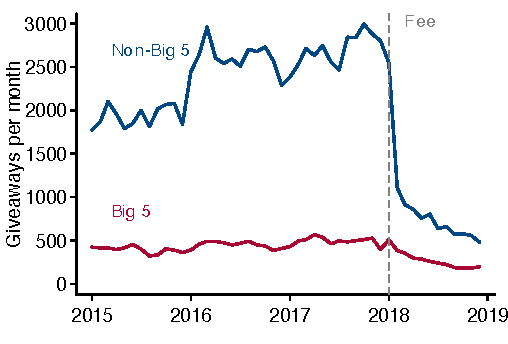
\includegraphics[width=\linewidth]{figures/giveaways_by_publisher.pdf}
      \source{Big 5: the five largest publishing houses.\\
      Giveaways per month, all publishers:\\
      about 3{,}200 in 2017, about 1{,}150 in 2018}
    \end{column}
  \end{columns}

\end{frame}

% ============================================================
\section{Table 2: Publishers}
% ============================================================

% Method
\begin{frame}{Table 2: 2017--18 vs.\ 2015--16 (DiD with a historical control group)}

  \vspace{-0.8em}
  \begin{center}
  \begin{tikzpicture}[
    lab/.style={font=\scriptsize, text=TextMid},
    brace/.style={decorate, decoration={brace, mirror, amplitude=4pt, raise=2pt}, thick, TextMid}
  ]
    \node[yr=SlateGray]    (y15) at (0,0)   {2015};
    \node[yr=UniBlueLight] (y16) at (2.3,0) {2016};
    \node[yr=SlateGray]    (y17) at (5.6,0) {2017};
    \node[yr=UniRedLight]  (y18) at (7.9,0) {2018};
    \foreach \n/\t in {y15/Before, y16/After, y17/Before, y18/After}
      \node[lab, above=1pt of \n] {\t};
    \draw[brace] (y15.south west) -- (y16.south east)
      node[midway, below=7pt, lab] {Control pair: no fee};
    \draw[brace] (y17.south west) -- (y18.south east)
      node[midway, below=7pt, lab] {Treated pair: \$119 fee from January 2018};
    \draw[UniRed, line width=1.6pt] ([yshift=-2pt]y18.south west) -- ([yshift=2pt]y18.north west);
  \end{tikzpicture}
  \end{center}

  \vspace{-0.8em}
  {\small
  \begin{equation*}
    \explain{y_{pt}}{giveaways by\\$p$ in month $t$}
    = \beta_1\,\explain{\text{Treated}_t}{$=1$ in 2017\\and 2018}
      \times\explain{\text{After}_t}{$=1$ in 2016\\and 2018}
    + \beta_2\,\text{Treated}_t\times\text{After}_t
      \times\explain{\text{Big5}_p}{$=1$ for Big 5\\publishers}
    \quad+\quad \explain{\delta_{m(t)}}{month-of-year\\fixed effect}
    \quad+\quad \explain{\sigma_{p,\text{pair}}}{publisher fixed\\effect per pair}
    + \varepsilon_{pt}
  \end{equation*}}

  \vspace{0.4em}
  \begin{columns}[T,onlytextwidth]
    \begin{column}{0.49\textwidth}
      \small
      \begin{itemize}
        \item 14{,}131 publishers $\times$ 48 months,\\
          all with a giveaway from 2016 on
        \item Big 5 = Penguin, HarperCollins, Hachette,\\
          Simon \& Schuster, Macmillan;\\
          the rest: indie and self-publishers
      \end{itemize}
    \end{column}
    \begin{column}{0.49\textwidth}
      \small
      \begin{itemize}
        \item $y$: (1) number of giveaways;\\
          (2) as a share of its 2015--17 total,\\
          which adjusts for publisher size
        \item $\beta_1$: 2018 change, non-Big 5;\\
          $\beta_2$: extra change, Big 5
        \item s.e.\ clustered by publisher
      \end{itemize}
    \end{column}
  \end{columns}

\end{frame}

% Results
\begin{frame}{Non-Big 5 publishers cut back twice as much, relative to their size}

  {\centering\footnotesize
  \begin{tabular}{@{}lcRcR@{}}
    \toprule
      & \multicolumn{2}{c}{(1) Number of giveaways} & \multicolumn{2}{c}{(2) Proportion} \\
    \cmidrule(lr){2-3}\cmidrule(l){4-5}
      & Paper & Replication & Paper & Replication \\
    \midrule
    Treated $\times$ After                & $-0.129$ (0.023)  & $-0.129$ (0.023)  & $-0.031$ (0.0004) & $-0.031$ (0.0004) \\
    Treated $\times$ After $\times$ Big 5 & $-43.354$ (6.561) & $-43.354$ (6.561) & $0.016$ (0.002)   & $0.016$ (0.002)   \\
    \midrule
    Observations                          & 678{,}288 & 678{,}288 & 611{,}376 & 611{,}376 \\
    $R^2$                                 & 0.883     & 0.883     & 0.038     & 0.038     \\
    \bottomrule
  \end{tabular}\par}

  \conclusion{The fee hits smaller publishers hardest, and the Big 5 gain share}

  \vspace{0.4em}
  {\small
  From 2017 to 2018, per publisher and month:
  \begin{itemize}
    \item Non-Big 5: 0.19 $\to$ 0.06 giveaways ($-68\%$)
    \item Big 5: 98.9 $\to$ 55.4 giveaways ($-44\%$)
    \item Scaled by own size (column 2): $-0.031$ vs.\ $-0.015$, about twice the cut
  \end{itemize}}

\end{frame}

% ============================================================
\section{Table 3: Genres}
% ============================================================

% Method
\begin{frame}{Table 3: popular, middle and niche genres (pre--post regression)}

  \vspace{-1.2em}

  {\small
  \begin{equation*}
    \explain{\text{Share}_{gt}}{genre $g$'s share\\of giveaway books\\in month $t$}
    \;=\; \beta_1\,\explain{\text{Post}_t}{$=1$ after\\the fee}
      \times\explain{\text{Top25}_g}{$=1$ if top 25\%\\(popular)}
    + \beta_2\,\text{Post}_t
      \times\explain{\text{Bottom25}_g}{$=1$ if bottom\\25\% (niche)}
    \;+\; \explain{\alpha_g}{genre\\fixed effect}
    \;+\; \explain{\delta_{m(t)}}{month-of-year\\fixed effect}
    + \varepsilon_{gt}
  \end{equation*}}

  \vspace{0.7em}
  \begin{columns}[T,onlytextwidth]
    \begin{column}{0.53\textwidth}
      \small
      \begin{itemize}
        \item 50 genres $\times$ 47 months, Jan 2016 to Feb 2020\\
          without Jan--Mar 2018
        \item Genre = a book's two most common shelves\\
          (tags readers assign, e.g.\ romance)
        \item Pre-fee share quartiles: 13 top (popular),\\
          24 middle and 13 bottom (niche) genres
        \item $y$: (1) raw share;\\
          (2) share relative to the genre's pre-fee mean
        \item $\beta_1$, $\beta_2$: change for top, bottom genres
        \item s.e.\ clustered by calendar month
      \end{itemize}
    \end{column}
    \begin{column}{0.44\textwidth}
      \centering
      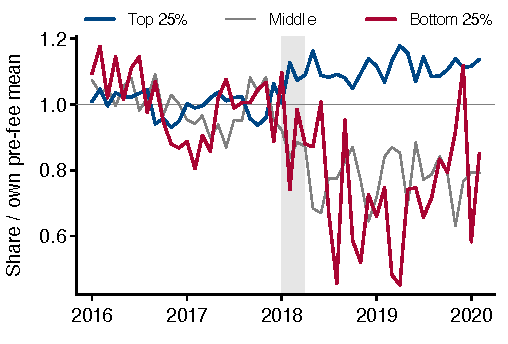
\includegraphics[width=0.95\linewidth]{figures/genre_shares.pdf}
      \source{Gray band: January--March 2018, dropped}
    \end{column}
  \end{columns}

\end{frame}

% Results
\begin{frame}{Popular genres gained 11\%; niche genres lost 26\% of their share}

  {\centering\footnotesize
  \begin{tabular}{@{}lcRcR@{}}
    \toprule
      & \multicolumn{2}{c}{(1) Raw proportion} & \multicolumn{2}{c}{(2) Percentage change} \\
    \cmidrule(lr){2-3}\cmidrule(l){4-5}
      & Paper & Replication & Paper & Replication \\
    \midrule
    Post $\times$ Top 25\% genre    & $0.012$ (0.001)   & $0.012$ (0.001)   & $0.110$ (0.010)  & $0.110$ (0.010)  \\
    Post $\times$ Bottom 25\% genre & $-0.001$ (0.0001) & $-0.001$ (0.0001) & $-0.262$ (0.039) & $-0.262$ (0.039) \\
    \midrule
    Observations                    & 2{,}350 & 2{,}350 & 2{,}350 & 2{,}350 \\
    $R^2$                           & 0.969   & 0.969   & 0.188   & 0.188   \\
    \bottomrule
  \end{tabular}\par}

  \conclusion{Genre diversity falls: popular genres gain share, niche genres lose it}

  \vspace{0.4em}
  {\small
  After the fee, each group's share relative to its own pre-fee mean:
  \begin{itemize}
    \item Top 25\%, popular (average share 10.5\% before): $+11\%$
    \item Middle 50\% (1.6\% before): $-22\%$
    \item Bottom 25\%, niche (0.34\% before): $-26\%$
  \end{itemize}}

\end{frame}

% ============================================================
\section{Table 4: Reviews}
% ============================================================

% Method
\begin{frame}{Table 4: pre- vs.\ post-fee cohorts (DiD with two-way fixed effects)}

  \vspace{-1.2em}

  {\small
  \begin{equation*}
    \explain{N_{jt}}{number of ratings of\\book $j$ in month $t$}
    \;=\; \beta_1\,\explain{\text{PostGiveaway}_{jt}}{$=1$ in the 12 months\\after the giveaway}
    + \beta_2\,\text{PostGiveaway}_{jt}
      \times\explain{\text{PostMon}_j}{$=1$ if the giveaway\\ran after the fee}
    \;+\; \explain{\alpha_j}{book\\fixed effect}
    \;+\; \explain{\gamma_t}{year-month\\fixed effect}
    + \varepsilon_{jt}
  \end{equation*}}

  \vspace{0.7em}
  \begin{columns}[T,onlytextwidth]
    \begin{column}{0.53\textwidth}
      \small
      \begin{itemize}
        \item 12 months before and after each giveaway;\\
          months without ratings count as 0
        \item Cohort = when the book's giveaway ran:\\
          58{,}677 before the fee, 22{,}931 after
        \item $\beta_1$: giveaway effect, pre-fee cohort;\\
          $\beta_2$: extra effect, post-fee cohort
        \item s.e.\ clustered by book
        \item Replicated: columns (3) and (4),\\
          the number of ratings
      \end{itemize}
    \end{column}
    \begin{column}{0.44\textwidth}
      \centering
      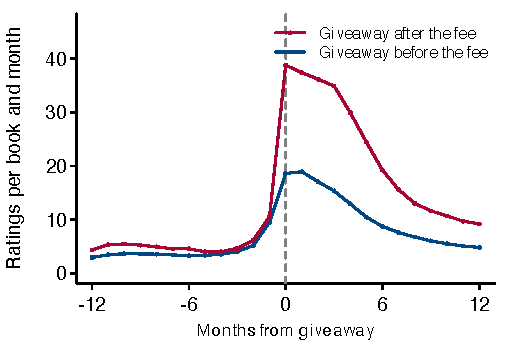
\includegraphics[width=0.95\linewidth]{figures/ratings_event_time.pdf}
      \source{Raw means, before fixed effects}
    \end{column}
  \end{columns}

\end{frame}

% Results
\begin{frame}{After the fee, a giveaway brought three times as many ratings}

  {\centering\footnotesize
  \begin{tabular}{@{}lcRcR@{}}
    \toprule
      & \multicolumn{2}{c}{(3) Number of ratings} & \multicolumn{2}{c}{(4) Number of ratings} \\
    \cmidrule(lr){2-3}\cmidrule(l){4-5}
      & Paper & Replication & Paper & Replication \\
    \midrule
    Post-Giveaway                   & $11.008$ (0.182) & $11.008$ (0.182) & $6.841$ (0.176)  & $6.841$ (0.176)  \\
    Post-Giveaway $\times$ Post-Mon &                  &                  & $14.454$ (0.372) & $14.454$ (0.372) \\
    \midrule
    Observations                    & 2{,}036{,}383 & 2{,}036{,}383 & 2{,}036{,}383 & 2{,}036{,}383 \\
    Adjusted $R^2$                  & 0.131         & 0.131         & 0.134         & 0.134         \\
    \bottomrule
  \end{tabular}\par}

  \conclusion{The fee amplifies the giveaway effect: more ratings, but lower scores}

  \vspace{0.4em}
  {\small
  After a giveaway, per book and month (sample mean: 9.37 ratings):
  \begin{itemize}
    \item Pre-fee cohort: $+6.8$ ratings
    \item Post-fee cohort: $6.8 + 14.5 = +21.3$ ratings, about three times as many
    \item Post-fee cohort's average rating: a further $-0.05$ stars (column 2, not replicated)
  \end{itemize}}

\end{frame}

% ============================================================
\section{Discussion}
% ============================================================

\begin{frame}{Discussion: one fee, traced across both sides of the market}

  {\centering
  \begin{tikzpicture}[
    node distance=0.34cm,
    tag/.style={font=\scriptsize\bfseries, text=UniBlue},
    arr/.style={-{Stealth[length=2mm]}, thick, TextMid}
  ]
    \node[chain=UniRed]                (fee) {\textbf{\$119 entry fee}\\ January 2018};
    \node[chain=UniBlue, right=of fee] (sup) {Small publishers cut back most};
    \node[chain=UniBlue, right=of sup] (gen) {Popular genres gain share};
    \node[chain=UniBlue, right=of gen] (dem) {More ratings, lower stars};
    \node[chain=UniBlue, right=of dem] (fit) {More bad reviews\\ from poor fit};
    \foreach \a/\b in {fee/sup, sup/gen, gen/dem, dem/fit} \draw[arr] (\a) -- (\b);
    \node[tag, above=1pt of sup] {Table 2};
    \node[tag, above=1pt of gen] {Table 3};
    \node[tag, above=1pt of dem] {Table 4};
    \node[tag, above=1pt of fit] {Table 5};
  \end{tikzpicture}\par}

  \vspace{0.5em}
  \begin{columns}[T,onlytextwidth]
    \begin{column}{0.48\textwidth}
      \colhead{What the paper adds}
        \footnotesize
        \begin{itemize}
          \item A fee changes \emph{who} stays and\\
            \emph{what} is promoted, not just how many join\\
            \parencite{rochet2003platform,armstrong2006competition}
          \item Fixed costs push out niche tastes:\\
            preference externalities \parencite{waldfogel2003preference}
          \item Deals bring more but less satisfied buyers:\\
            the Groupon effect \parencite{byers2012groupon}
          \item The fee selects on budget, not quality:\\
            post-fee books were not rated higher before
        \end{itemize}
    \end{column}
    \begin{column}{0.48\textwidth}
      \colhead{How to read the estimates}
        \footnotesize
        \begin{itemize}
          \item The fee hit all at once: Tables 2--3 are\\
            before--after changes, net of seasonality
          \item Table 4 compares cohorts: $\beta_2$ mixes\\
            which books enter after the fee\\
            with how readers respond to them
          \item All three tables reproduce exactly\\
            from the authors' data
        \end{itemize}
    \end{column}
  \end{columns}

\end{frame}

% End slide
\WhartonEndFrame

% Appendix: references, not counted in the page total
\appendix

\begin{frame}{References}
  \nocite{zhu2025monetizing}
  \printbibliography[heading=none]
\end{frame}

\end{document}
